% Authorship: Claude-drafted, author-revised
\section{Practice Is Not Unitary}

Part V settled a question of possibility with the simplest mechanism
available and left open the question this Part makes central. Asked to
confer weight on the same principles, do the several mechanisms of
practice confer the same weight? They do not. That is the second of
this Article's two findings. The first, from Part IV, was that the stipulated engine is sound: given
faithful weights, the weighted sum weighs magnitude, tolerates rough
specification, and leaves more law standing than the hierarchical Hart. On the
evidence below, that engine is sound in a way
that does not settle legal content, because it does not settle which
practice supplies the weights, and different practices supply different
ones.

In four steps, each turning on the one before it, the argument runs as
follows. All four mechanisms of practice clear the same bar, three of them on
every seed and appointment on twenty-six of thirty for noise tolerance. That no
mechanism fails is worth establishing, though the four requirements differ
sharply in how much they discriminate, and only noise tolerance separates the
mechanisms. Yet the four mechanisms ground the principles
differently, into weight structures that collapse to three rather than four
because two of them converge. Run over the same disputes, those structures then decide real cases
differently, reaching different verdicts about a third of the time and
opposite determinate verdicts about a quarter of the time. From
this it follows that principled positivism does not resolve the
indeterminacy it inherited from Hart and Dworkin. It relocates the question from how principles combine, settled in
Part IV, to the practice that grounds the weights, left open by the
theory.

\subsection{Four Mechanisms, One Bar}

Between them, the four mechanisms model four readings of what it is for a
principle to be taken up in practice. \textit{Uptake}, the mechanism of Part V, reads
taking-up as invocation frequency: a principle earns weight in proportion
to how often the bench reaches for it. \textit{Reliance} reads it as earned authority: a principle
gains weight by prevailing in contested disputes and by embedding itself in the holdings that go on relying on
it. \textit{Strategic} reads it as convergence under interaction:
reinforcement-learning judges, adjusting to one another, settle toward a
shared weight. \textit{Appointment} reads it as institutional inheritance:
with a near-random turnover of the bench, a principle's weight is the
decayed breadth of the still-live holdings that support it.\footnote{The appointment dynamic is not drawn from Berman's published text. It responds to his suggestion, in correspondence, that the turnover of the bench is a further channel through which practice fixes weight. E-mail from Mitchell N.\ Berman to author (Mar.\ 2026) (on file with author); see \textit{supra} Part~III.A.} Part III describes the four in full. For present purposes the point is that
each is a \textit{construal} of one phrase in Berman's account, ``taking-up,''
meaning a way of settling what that phrase picks out in a practice, and that
the four are genuinely different construals rather than variations on one.\footnote{Berman, \textit{Practices}, \textit{supra} note 7, at 329
(principles are ``constituted by the taking-up behaviors of the system's
subscribers''); see also \textit{id.}\ at 320 (fundamental legal principles
are ``grounded in practices ... by dint of legal actors taking them up in
legal decision-making'').}

That last claim carries the whole of this Part, and it needs more than one
sentence to bear it. Set each mechanism beside the text it construes.

\textit{Uptake} takes Berman at the point where he locates the constituting
relation. As he writes, principles are ``constituted by the taking-up
behaviors of the system's subscribers.''\footnote{\textit{Id.}\
at 329.} There, taking-up is described as something officials do, repeatedly, in the
course of deciding cases. Of the readings available, counting how often they do it is arguably the
most direct thing a model can make of that sentence, and it is the reading
Part V implements.

\textit{Reliance} takes up a second commitment, one Berman has pressed
harder in the later work: a principle is embedded by the holdings that go
on relying on it, so that it does not forfeit its standing the moment it
stops being mentioned.\footnote{Berman, \textit{Practices},
\textit{supra} note 7, at 310--14 (a principle embedded by the holdings
that rely on it retains vitality without current invocation); Berman,
\textsc{To Say What the Law Is}, \textit{supra} note 7 (manuscript ch.\
6).} Written out as a rule of accrual, that commitment becomes a dynamic that
confers weight for prevailing in contested dispositive disputes, amplifies
the gain by how much the resulting holding is later relied upon, decays it
over time, and strips it on overruling. Part
III calls reliance the closest of the four to Berman's own account, and
nothing in this Part revises that.

\textit{Appointment} is his in the plainest sense: he proposed it. Told
that the project modeled uptake and strategic adaptation, he replied that
the turnover of the bench is a further channel through which practice
fixes weight.\footnote{E-mail from Mitchell N.\ Berman to author (Mar.\
2026) (on file with author); see \textit{supra} Part~III.A.} To the embedding point the mechanism joins that suggestion, reading a
principle's vitality off the still-live holdings that support it rather
than off its current invocation.

\textit{Strategic} is the weak member of the set, and Part III already
says so, calling it the least Bermanian of the four, since Berman nowhere
describes judges optimizing toward a goal, and reinforcement learning brings with it a picture of adjudication he
seems not to hold.\footnote{\textit{Supra} Part~III.A (of the four mechanisms strategic is the
least Bermanian, and should be read as a robustness lens rather than as an
interpretation of the theory).} As a robustness lens, though, it arguably earns its place. Weights produced by a process Berman would not endorse, clearing every
requirement he does endorse, suggest that the requirements are not an
artifact of any one picture of practice. That is the whole of what
strategic is asked to do.

Three of the four have a warrant in Berman, then, and one is a lens. A reader
declining the lens can read the Part with uptake, reliance, and appointment
alone. With strategic dropped, a later Section reports the finding, and it looks much
the same.

Held to the four requirements of Part III across thirty seeds, every
mechanism passes, three on every seed and appointment on twenty-six of thirty for
noise tolerance.\footnote{Appointment counts as passing that requirement under
the seed share Part III states, which asks $0.80$ of seeds on noise tolerance
against $0.90$ on the other three. At the stricter share it would not clear
it. The asymmetry is in the implementation rather than in anything Berman
claims, and it is disclosed here because appointment is the only mechanism it
touches.} Each produces weights that are well-defined, that survive weight error up to
Part III's floor, that weigh magnitude rather than counting principles
lexically, and that leave a positive determinacy margin over the hierarchical
Hart. The margins sit near the stipulated engine's own advantage of about
$+0.27$: uptake near $0.27$, reliance $0.291$, strategic $0.283$, appointment
$0.284$.\footnote{Those four figures are closer together than they look. The
hierarchical Hart consults the activations and the category tiers and never
the weights, so on a given case draw it returns the same determinacy rate
whichever mechanism it is set against. Each margin is that mechanism's own
determinacy rate less one shared constant, and the weighted sum's determinacy
rate varies little across weight vectors. The clustering is therefore close to
arithmetic rather than a convergence of four independent measurements.} In the
mean, noise tolerances run from about $0.084$ to $0.097$, though the means
understate how tight the requirement is. Since it is scored seed by seed,
the binding figure is each mechanism's worst run: $0.085$ for uptake,
$0.078$ for reliance, $0.073$ for strategic, and $0.067$ for appointment,
against a floor of $0.07$.

One mechanism clears noise tolerance only barely, though, and the honest course is
to say so rather than smooth it over. Appointment meets three requirements on
every seed but meets noise tolerance on only twenty-six of thirty, its
critical uncertainty $\sigma^{*}$, the level of Gaussian weight perturbation at
which one case in five flips its signed verdict, straddling the $0.07$ floor
(minimum $0.067$, median $0.085$). That a near-random mechanism, one with no selection of any kind, only just
clears that floor is some evidence that noise tolerance is doing work. It
would be a mistake, though, to read appointment's near-miss as evidence that
the other three passes were hard-won, and the point is worth making against
this Article's own interest.

Of the four requirements, only noise tolerance discriminates among weight
vectors at all. Well-definedness asks that at least two principles carry
weight above a small cutoff, a condition almost any vector satisfies. The
magnitude probe compares the weighted sum against a lexical rule, so it tests
the aggregation form rather than the weights the form is given.
And the hierarchical Hart never reads the weights, so a positive margin over
it follows from the weighted sum deciding more cases than a tiered rule does,
as it will for almost any weights. Drawing weight vectors uniformly at
random and scoring them confirms this: on five hundred random vectors the
well-definedness test passes five hundred times and the Hart comparison five
hundred times, at margins from $+0.07$ to $+0.29$, and on a sixty-vector
subset the magnitude probe passes sixty times, never at less than nine times
the
lexical rule's rate against the five-fold bar.\footnote{Scored on the same
eight-hundred-case held-out battery the mechanisms are scored on. Even a
degenerate vector placing all weight on one principle returns a Hart margin of
$+0.19$. The hierarchical Hart's determinacy rate is bit-identical under a
zero vector and a random one, which is what one would expect of a rule that
never consults the weights.}

So three of the four requirements are properties of the aggregation form
rather than tests of a mechanism's output, and every mechanism inherits that
form by construction. Only noise tolerance asks something of the weights
themselves, and it is the one requirement that separates the four mechanisms.
The robustness result of this first step is therefore narrower than it first
appears. The formal machinery survives every picture of practice, and that is
Part IV's finding rather than a new one. The four mechanisms
are shown to share a minimum rather than a standard. This does not weaken the
Part's argument. A test that four incompatible construals all clear is a test
that cannot choose between them.

For its soundness, the weighted sum does not depend on any one picture of how
weight is conferred. That is the setup for the difficulty that follows: soundness under
every mechanism is not agreement across mechanisms.

\subsection{Three Structures, Not Four}

On the requirements the four mechanisms agree, and about everything else
they disagree. Each confers not a scalar quality of legality but a
\textit{structure}: a full vector of weights across the nine principles,
saying which count for much and which for little. Those structures diverge
sharply, and in a way that Figure \ref{fig:f2-practice} makes visible at a
glance.

\begin{figure}[t]
\centering
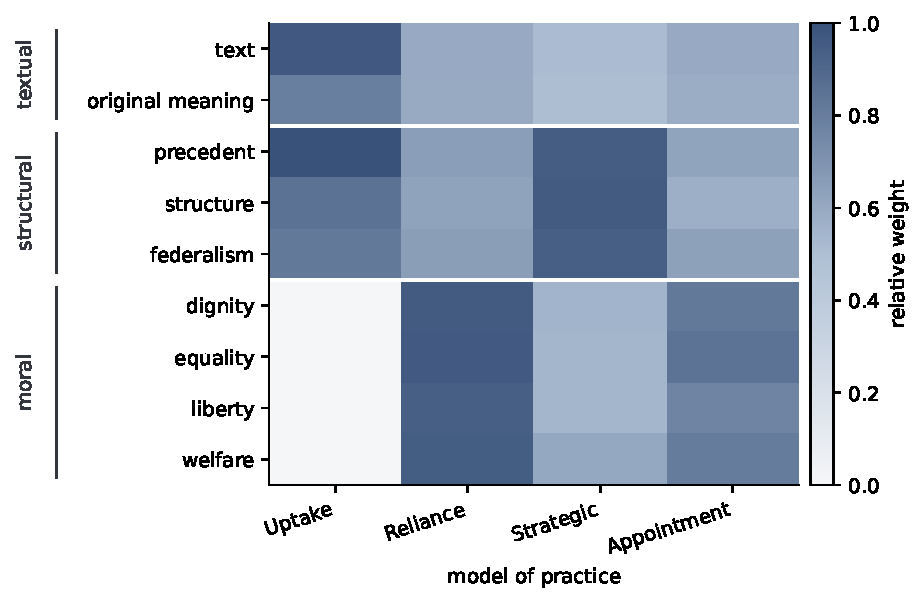
\includegraphics[width=\textwidth]{F2_practice_not_unitary}
\caption{Practice is not unitary. Across the nine principles, each column is one mechanism's emergent weight
structure; darker cells carry more weight. All four mechanisms clear the four requirements of Part III.
Uptake concentrates on the textual and structural principles and drives
the four moral principles to zero; reliance and appointment lift the
moral principles highest; strategic lifts the structural principles
highest. Reliance and appointment converge (rank correlation $+0.93$),
so the four dynamics realize three distinct structures, not four.
Appointment is the marginal mechanism on noise tolerance, clearing it on
twenty-six of thirty seeds. The heavier moral tier under reliance and
appointment is partly a category-size effect: the moral tier holds four
principles to the structural tier's three and the textual tier's two, so
under correlated activations it accrues broader aggregate force.}
\label{fig:f2-practice}
\end{figure}

Read down the columns and the structures are plainly different. Under \textit{uptake}, weight collects on
the textual and structural principles, text at $0.96$, precedent at
$1.00$, original meaning at $0.79$, structure at $0.85$, federalism at
$0.82$, while all four moral principles, dignity, equality, liberty, and
welfare, fall to zero. Of the four, uptake produces much the most concentrated
structure, its coefficient of variation, meaning spread relative to the mean,
near $0.90$. That figure is read off the vector after the live/dead cut, applied by
no other mechanism, so it chiefly registers the distance
between five live principles and four zeros rather than gradation among the
live five. Among those five the weights run from $0.79$ to $1.00$ and their coefficient
of variation is $0.09$, tighter than any other mechanism manages.

Under \textit{reliance}, the ordering nearly inverts: the moral principles sit
highest, dignity at $0.95$, equality at $0.96$, liberty at $0.94$, welfare
at $0.95$, while the textual and structural principles settle in the low
sixties. Against uptake, reliance spreads its weights far more evenly, its coefficient of
variation near $0.24$. Under \textit{strategic}, the structural principles lead, precedent at $0.94$,
structure at $0.96$, federalism at $0.94$, with text and original meaning near
$0.50$ and the moral principles in the middle, a coefficient of variation near
$0.35$. Those figures are from the methodology-seeded start, the
configuration the four-way comparison uses throughout; from a neutral start
the same bench settles on a different structure, as the end of this Section
reports.
Under \textit{appointment}, the moral principles again lead, dignity
$0.82$, equality $0.85$, liberty $0.77$, welfare $0.80$, but the whole
structure is the flattest of the four across all nine principles, its
coefficient of variation near $0.155$.

In every case these headline dispersions are the per-seed means, not the
dispersion of the averaged vectors, so they report how concentrated each
mechanism is on a typical run rather than an artifact of averaging.

Behind each of those structures lies a cause, and naming them keeps the
finding from reading as the claim that different code returns different
numbers.
Part V gave uptake its causal account: the bench is composed in equal
quarters of four methodologies, two of them reaching for the textual and
structural principles far more often than for the moral ones, so the moral
principles accumulate the fewest invocations, while the heaviest accumulations
fall to the principles the bench as a whole will take up rather than to those
any one methodology favors. The sensitivity analysis locates uptake's structure in exactly that
composition. Of the parameters the uptake model takes, the spread of
invocation tendencies across the methodologies accounts on its own for
about half the variation in the mechanism's output, a first-order
index of $0.52$.\footnote{Two different statistics are involved, and they are not
comparable. For uptake and reliance the figure is a first-order Sobol
index: the share of the variation in a mechanism's emergent weights
attributable to one parameter varying on its own, which runs from $0$ to
$1$. Those indices are $0.52$ for the spread of invocation tendencies under
uptake and $0.91$ for the clash threshold under reliance. Strategic trains
a network at every evaluation, which makes a Sobol decomposition too
costly, so it was screened by Morris elementary effects instead. Its $0.20$
for the learning rate is a mean absolute effect on the raw output scale,
not a variance share, and it is not bounded above by one. It supports a
ranking of that mechanism's own parameters and no comparison across
mechanisms. Appointment is described in the text from its construction
rather than from a dominant parameter. A high index locates where a
mechanism's output comes from; it is not by itself a defect, since a
mechanism has to depend on something.} Uptake counts invocations, and
this bench's mix of methodologies invokes the textual and structural
principles most.

Reliance depends on something quite different, and more sharply. Its
structure turns almost entirely on the disputes counted as contested. The
clash threshold, the line separating a genuine
conflict from a case that decides itself, carries a first-order Sobol index of $0.91$ against uptake's $0.52$, the only
two computed that way, and the dependence follows
from the object the mechanism reads. Reliance confers weight
on the principles that prevail in contested, dispositive disputes, so
where the line around ``contested'' falls decides which disputes are eligible
to confer weight at all. Moving that line does not adjust the mechanism's sensitivity. It changes
the population of cases from which weight can be earned.

Appointment's structure follows from its read-out rather than from any
single parameter. It measures holding-support, the decayed breadth of the
still-live holdings resting on each principle: survival rather than mention. Under that read-out, a principle no one has invoked lately keeps its weight
for as long as the holdings built on it stand, and a principle invoked
constantly gains nothing until an invocation becomes a holding that
lasts.

Strategic's structure traces most to its learning rate, ranked first among its
four parameters by the Morris elementary-effects screen. Because that
screen returns a different statistic, the figure cannot be set beside
uptake's or reliance's, and the claim available here is the weaker one: within
strategic, no single parameter dominates the others as the clash threshold
dominates under reliance. What strategic rewards is decisive consensus. That would tend to favor the
principles a bench of mixed methodologies can actually agree on, and
those are the structural ones. That absence of a dominant parameter
is also why the starting configuration matters as much as it
does, a point the end of this Section returns to.

Set side by side, the four accounts are not variations on one account.
Uptake tracks how often a principle is reached for. Reliance tracks the
outcome of the disputes that a threshold marks as real. Appointment
tracks what survives. Strategic tracks what a divided bench can settle
on. Taken singly, each is an intelligible reading of practice conferring
weight, and each seems to measure a different thing about the practice. That is why the
structures differ: the four mechanisms are not four implementations
disagreeing about one quantity; they are four quantities.

Read against one another, the four dynamics reduce to three. The
pairwise rank correlations between the mean weight vectors sort the
mechanisms cleanly. Uptake stands opposite reliance
($-0.78$) and opposite appointment ($-0.75$): what uptake elevates,
those two suppress. Strategic sits apart from the other three, weakly positive with uptake ($+0.31$),
weakly positive with reliance ($+0.15$), and near zero with appointment
($-0.08$). By contrast, reliance and appointment
all but coincide, their rank correlation $+0.93$. Two mechanisms built to different specifications, one rewarding winners in
contested disputes and one inheriting holdings across a near-random bench,
converge on the same ordering of the principles. They are not strangers to one
another, and the convergence is less surprising for that: both draw their
exogenous pressure structure, the fixed pattern of decision pressure that
settles disputes from outside the weight dynamic, from the same source on a
given seed, both skip
cases the weighted sum leaves indeterminate, and both credit a principle by
the same test, prevailing on the winning side by a
margin.\footnote{The appointment mechanism was built with the reliance
mechanism in view, and the shared construction is why the second caution below
matters. What the convergence shows is not that two unrelated dynamics
coincide but that two readings of taking-up which both look to holdings
deliver the same ordering.} On that reading the four
mechanisms realize three structures: uptake alone, strategic alone, and the
reliance-appointment pair as one.

Three cautions keep this from being overclaimed, and none is a formality. The
first is that the correlations are noisy across seeds, so the reduction to
three should not rest on the averaged figures alone. The uptake-reliance
opposition holds up well: its per-seed mean rank correlation is $-0.68$ with a
standard deviation of $0.25$, strongly and consistently negative, if not the
clean $-0.78$ of the averaged vectors. The reliance-appointment convergence holds up
too. One pair does not. On the averaged vectors reliance and strategic correlate at $+0.15$, and at
$-0.20$ per seed, so that pair's sign is an artifact
of averaging and nothing should be read off it.\footnote{Per-seed mean
$-0.201$, standard deviation $0.388$, running from $-0.717$ to $+0.783$ across
seeds. The two averaged-vector estimators disagree with each other on this
pair as well, the rank correlation coming out at $+0.15$ against a linear
correlation of $-0.45$. It is the noisiest pair in the study, and the
reduction to three structures does not turn on it: strategic sits apart from
the other three on any of these readings.} So the convergence and the
opposition are properties of the runs rather than of the averaging, but that
is a claim about the two pairs the argument uses, not about every cell of the
matrix.

The second caution is the sharpest, and the Introduction promised it: the
convergence is measured on a bench where both mechanisms read a common
legal culture, the design this Article defends. A single legal
system is one culture, and modeling two mechanisms as reading different
ones would answer a question nobody asked. For the convergence claim, though, the choice is load-bearing.
Decouple the cultures, so that reliance and appointment each read their
own, and the rank correlation falls from $+0.833$ to $+0.302$, and its
dispersion across seeds rises from $0.096$ to $0.451$, with two of eight
seeds turning negative.\footnote{This decoupling test is a separate run, and its baseline is not the $+0.93$
reported above. The $+0.93$ is a single rank correlation between the
thirty-seed mean weight vectors; the figures here are means of eight per-seed
rank correlations. The drop is therefore measured from $+0.833$, not from
$+0.93$. Eight seeds. Shared culture $\rho = +0.833$ (sd $0.096$); independent
cultures $\rho = +0.302$ (sd $0.451$), with seed-level values running from
$-0.533$ to $+0.850$. The convergence
therefore tracks the shared culture at least as much as it tracks the
shared object read. Both readings survive: what the two mechanisms have in
common is that they read holdings, and that they read holdings deposited by
the same practice.} On that showing, the pair share not only the object they read but
the practice that deposits it. That narrows the convergence claim
without dissolving it. Here again the structures
are properties of these runs rather than laws about practice.

The third caution is that under reliance and appointment the shared moral
lean is likely in part a category-size effect rather than a pure agreement
of substance. The moral
tier holds four principles where the structural tier holds three and the
textual tier holds two, so under the correlated activations of realistic
cases the moral tier accrues broader aggregate force simply by being
larger.\footnote{Both mechanisms generate their weights on a category-correlated case stream,
where uptake's is independent. \textit{See supra} Part~III.A. Rerunning
reliance on an independent stream leaves the direction of its moral lean
intact while removing most of its size, so the caution about reliance concerns
how large the lean is rather than whether it is there. The same test has not
been run for appointment.} That same size effect helps drive the $+0.93$ convergence.

The structure in which the moral principles lead is reachable by more than one
route, so it is sensitive
to what one assumes at the outset about which principles belong together. That is a
reason to report three structures as a finding about the mechanisms rather
than as a law about practice.

Those cautions limit the convergence. They do not exhaust it. There is a
further reading of why reliance and appointment coincide, and it is perhaps
worth stating as a finding rather than leaving as an accounting note. In their rules of conferral the two mechanisms have almost nothing in common.
One rewards principles that prevail in contested, dispositive disputes and
amplifies the gain by how much the resulting holding is later relied on. At
intervals, the other replaces a random cohort of the bench and reads weight off
the decayed breadth of the still-live holdings that rest on each principle.
For all the simulation scaffolding the two share, neither rule was drawn from
the other. What they do share is the object they read. Both read holdings. Uptake
reads invocations.

That distinction is Berman's own, and he has pressed it. On his account a
principle is taken up when officials reach for it in their reasoning, and
it is embedded when the holdings relying on it continue to stand, so that
its vitality does not depend on its being currently invoked.\footnote{Berman, \textit{Practices}, \textit{supra} note 7, at
302 (taking-up); \textit{id.}\ at 310--14, 321--22; Berman, \textsc{To
Say What the Law Is}, \textit{supra} note 7 (manuscript ch.\ 6) (a
principle is embedded by the holdings that continue to rely on it, and
disavowal is distinct from mere desuetude); E-mail from Mitchell N.\
Berman to author (Mar.\ 2026) (on file with author); see \textit{supra}
Part~II.D. The convergence at issue is a rank correlation of $+0.93$
between the mean reliance and appointment weight vectors and a verdict
disagreement of $1.8\%$ on the fifty-thousand-case common battery reported
in Section~VI.C.}
Read that way, the reduction from four dynamics to three is not two
implementations happening to land near each other. It would seem to track a
line the theory already draws. Where the mechanisms read what officials say,
they produce one structure; where they read what officials' decisions leave
standing, they produce another. The distance between those two is the
widest in the study: the rank correlations just reported, negative
between uptake and each member of the holdings-reading pair against
$+0.93$ within it, and, as the next Section reports, the largest verdict
divergences the four mechanisms produce.

If the reading holds, this Part leaves open something sharper than a choice
among four models. It leaves open a choice between invocation and
embedding as the ground of weight. That is a question about the kind of
practice that grounds legal content, and one on which Berman's own text
points both ways at once.

Two limits attach. The first is that this is an interpretation of a
convergence between two mechanisms rather than a test that separates
invocation from embedding.
Establishing it would take a design that varied the object read while
holding the rest of each mechanism fixed. That is not the design run here. The second is that the reading does not accommodate strategic. Reading neither
invocations nor holdings but the agreement a bench can reach, strategic
sits apart from the other two structures. Separately, the category-size effect noted
above and this reading are not exclusive. Both may be operating, and
these runs cannot apportion the $+0.93$ between them.

Even a single mechanism need not fix a single structure. The strategic mechanism's tier-lean depends on where its judges begin. Started from a
methodology-seeded configuration, the strategic bench converges toward
the structural principles, with structural weight above $0.90$. Started
from a neutral configuration, the same bench converges toward the moral
principles, with moral weight above $0.90$. The precise crossover point between the two regimes is
machine-fragile, and no figure is reported for it. Even so, the qualitative fact
appears robust, and it sharpens the
Part's claim. Not only do the four mechanisms disagree with one another, but even one
taken alone is not a single fixed structure. Its output turns on a starting point that
practice does not hand us.

\subsection{The Difference Decides Cases}

Two cases show what the rates below are made of. Both have already been worked in this Article: \textit{TVA v.\ Hill}, used in
Part II to introduce the model, and \textit{Obergefell v.\ Hodges},
used there to illustrate outweighing. Run through the four
mechanisms' emergent weight vectors, each turns the divergence from a
percentage into a disposition.

Before the numbers, a word about what they are. The \textit{TVA}
activations are Berman's own, taken from his figures for that case and
reported in Part II. By contrast, the \textit{Obergefell} profile is mine, built from the
principles he identifies as bearing on that dispute. Both are
illustrative rather than empirically coded: they show how the model
works, not how strongly each principle in fact bore on either
dispute.\footnote{Berman, \textit{Practices}, \textit{supra} note 7, at
338--42 \& figs.\ 8--9 (the \textit{TVA} activations, reproduced
\textit{supra} Part~II.B \& tbl.~\ref{tab:tvah}); \textit{id.}\ at
330--36 (the illustrative principle set). The \textit{Obergefell} profile
assigns activations to the principles Berman treats as engaged there and
is my construction, not his; it is offered as an illustration and nothing
in this Part turns on the particular values, as the perturbation test
below reports.}
No finding in this Part rests on them. The divergence rates reported below come from fifty thousand synthetic
cases, not from two real ones. The two cases supply a picture of
what a divergence of that size would look like when it lands on a docket.


In design this experiment is the mirror of Part II's. There, a single weight vector
was held fixed while the activations varied across two Justices. That is
Berman's own experiment: Burger and Powell read the same statute
differently, and the model locates their disagreement in the
activations. Here one activation profile is held fixed while only the
construal of practice varies. Same case, opposite experiment. The symmetry is worth stating, because it makes the stake plain. If Berman is
right that officials largely converge on the weights and divide over
activation, then holding the activations still ought to hold the verdict
still.

Since it is the place where a thumb could rest on the scale, the mapping from
Berman's labels to the canonical nine principles has to be stated.
Across the two diagrams Berman codes seven principles. Three of them need a
canonical home: congressional intent enters as original meaning, the
pursuit of happiness enters as liberty, and majoritarianism enters as
structure. Of the remainder, three map directly, and one, the avoid-absurdity
principle of the \textit{TVA} diagram, has no exact counterpart among the
nine. I place it with the general-welfare principle, as arguably the
closest of the nine to a consequence-regarding consideration. Because Berman does not code them and I have not supplied them, equality
and federalism go unactivated in both cases, and welfare in
\textit{Obergefell}. No activation was
added, dropped, or rescaled to produce what follows.\footnote{Placing
avoid-absurdity with welfare has a consequence worth naming, since it
runs in the direction of the result reported below: uptake assigns the welfare
principle no weight, so Burger's only consideration cutting against
prohibition drops out of uptake's sum entirely, which widens uptake's margin
over the other three. It does not produce that margin. Uptake returns the
largest figure under every placement tested, because its weights on the
textual and original-meaning principles are the highest of the four. The placement is a live
choice rather than a settled one. It does not disturb \textit{TVA} under
Burger, whose avoid-absurdity activation of $-0.2$ can move any total by
at most $0.2$ and leaves the unanimity intact under every placement
tested. It does disturb Powell's profile in the same case, whose
avoid-absurdity activation of $-0.9$ carries far more weight: that
profile also splits the mechanisms, but the split survives only nine of
thirteen alternative placements, and it is therefore not reported here.}

Take \textit{TVA} first, on Chief Justice Burger's reading. Here all four mechanisms agree, and none of them is close to the determinacy
threshold: uptake returns a
net force of $+1.499$, appointment $+0.836$, reliance $+0.821$, and strategic
$+0.741$. On every construal of practice, the law prohibits completing the
dam. Between them the mechanisms differ in the size of the force by a factor of
two, and nothing turns on the difference, because the verdict is the same
and the margin is comfortable under each. This is the ordinary case, what about two-thirds of the caseload looks like,
and it is worth seeing first.

\textit{Obergefell} is the other kind. Table~\ref{tab:mechanism-cases}
sets the two side by side. Under uptake the net force is $-1.154$, and the law runs against the
claimed right. Under reliance it is $+0.708$ and under appointment
$+0.509$, and the law runs for it. One case, one profile of activations, three faithful readings of what it is for a
principle to be taken up in practice, and the answer moves from one side
to the other. Strategic returns $-0.140$. At this Article's determinacy threshold of $0.2$
that is not a verdict at all but a gap: strategic declines to settle the case
the other three settle, uptake one way and reliance and appointment the other. On the bare sign of net force it
would lean with uptake. It should be taken as a case the threshold controls
rather than as a third kind of answer. Part VIII tests how much turns on where that
line falls.

\begin{table}[t]
\centering
\small
\caption{One activation profile, four construals of practice. Net force
under each mechanism's emergent weight vector, with the activations held fixed. Positive favors prohibition in \textit{TVA} and
the claimed right in \textit{Obergefell}.}
\label{tab:mechanism-cases}
\begin{tabular}{lcc}
\toprule
\textbf{Mechanism} & \textbf{\textit{TVA} (Burger)} & \textbf{\textit{Obergefell}} \\
\midrule
Uptake      & $+1.499$ & $-1.154$ \\
Reliance    & $+0.821$ & $+0.708$ \\
Strategic   & $+0.741$ & $-0.140$ \\
Appointment & $+0.836$ & $+0.509$ \\
\bottomrule
\end{tabular}
\end{table}

The split does not depend on the particular activation values assigned. Perturb every activation in the \textit{Obergefell} profile with
Gaussian noise and re-run the four mechanisms: uptake still opposes
both reliance and appointment on $100.0\%$ of draws at $\sigma = 0.05$,
on $99.1\%$ at $\sigma = 0.1$, and on $87.5\%$ at $\sigma =
0.2$.\footnote{Twenty thousand draws at each noise level. Each draw adds
independent Gaussian error to all nine activations and recomputes the
net force under all four mean weight vectors; the reported share is the
share of draws on which uptake's signed verdict opposes both reliance's
and appointment's. Activations run on the interval $[-1,+1]$, so
$\sigma = 0.2$ perturbs each activation by a tenth of the available
range in the typical draw.} At the largest of those perturbations the coding would have to be wrong by
a substantial margin on every principle at once, and even then the
opposition survives on seven draws in eight. However one judges the
coding, the disagreement among the mechanisms is probably not built out of
it.

The strongest thing here needs no coding assumption at all. Under uptake
the four moral principles carry weight exactly zero. Whatever their
activations, dignity and liberty therefore contribute nothing to the sum in
\textit{Obergefell}. Under uptake, Justice Kennedy's argument, that the originalist objections
were outweighed rather than invalid, cannot be run at all, because nothing
is available to do the outweighing. Uptake decides the case entirely on the textual and structural principles,
then.
Since each of the four moral principles is multiplied by zero before any judgment about its strength is consulted, no
judgment about how strongly dignity or liberty applies to same-sex marriage
can move the result. That follows from the weight vector
alone and would hold for any activation profile anyone cared to code.

The natural objection is that this makes the uptake result trivial. As a
matter of arithmetic, a mechanism that zeroes the moral principles will
decide a case about dignity on other grounds, so the conclusion is already
in the weights. The objection seems right as a description and wrong as a
dismissal. The weights were not stipulated. They emerged, and Part V traced their
source. Two qualifications keep the point honest.

In the first place, the zeros are the weights after the cut that separates
live principles from dead ones; the underlying
uptake shares are not zero but small, running from about $0.35$ to about
$0.50$ against $0.79$ to $1.00$ for the textual and structural
principles, and Part V reports that where the cut falls governs how many
principles count as live. The argument needs only the smallness, not the
literal zero: on the raw shares the moral tier still carries roughly
half the weight of the textual one, and \textit{Obergefell} still comes
out against the claimed right.

In the second place, the moral principles are weak under uptake because
this bench takes them up rarely, a modeled feature of the practice
being represented rather than an implementation artifact. Part V does
report a composition sweep where reseating the bench so that the
purposivist methodology holds a majority moves three principles across the
line. If taking-up is invocation frequency, then dignity is not a weighty
principle in this practice, and that would be a claim about the law. A
theory that grounds weights in practice owes an account of why the
implication is wrong. Berman may well have one, since embedding in
holdings is exactly the resource such an account would draw on, and that
is the reliance mechanism, deciding \textit{Obergefell} the other
way.

That is the shape of the finding stated case by case. \textit{TVA} falls
among the cases where the construal of practice is idle, and
\textit{Obergefell} among the cases where it decides. The $36.1\%$
reported next measures how often each happens.

If they agreed on outcomes, distinct structures would be a curiosity. They
do not. Run over a common battery of fifty thousand synthetic cases, the four mean
weight structures reach \textit{different} verdicts on $36.1\%$ of cases on
the bare sign of net force, and on $44.5\%$ once the determinacy threshold this
Article uses throughout is applied. On $27.2\%$ of cases some pair reaches
\textit{opposite determinate} verdicts, one construal saying the law points
one way and another saying it points the other.\footnote{Each of the four mean
weight structures is run over the same fifty thousand synthetic cases, once
with category-correlated activations and once with independent activations, as
defined in Part~IV. The $36.1\%$ compares bare signs and so counts a case as
disagreed whenever the structures fall on different sides of zero; the
$44.5\%$ counts them as disagreed whenever their gated verdicts differ, which
includes a case where one structure decides and another abstains. The
opposite-determinate figure is a share of all fifty thousand cases; among the
$73.5\%$ on which all four structures are determinate, the share is $24.8\%$.
The runs are reproducible from the code and data repository accompanying this
Article.} These are the measured backbone of the second finding.

The figures reported here are the correlated-activation ones, the realistic
case being one in which principles in the same category tend to fire together.
On independent activations, the conservative baseline that Parts IV and V used as
their stress test, the bare-sign disagreement is $31.8\%$, the gated
disagreement $42.5\%$, and the opposite-determinate rate $19.9\%$. Even at that
baseline, about one case in five sees two construals reach determinate verdicts
pointing opposite ways. The design cannot say how that share would move on a
real docket.

One caveat governs all of these figures. They are computed on the four mean
weight vectors, each averaged across thirty seeds, rather than on the runs
those means summarize. Averaging smooths seed-to-seed variation, so the
figures describe how four idealized structures relate to one another rather
than how any four particular runs do.

The honest counterpart to those figures is that a majority of cases are not
affected. On the bare sign the four structures agree about two-thirds of the
time, and at the determinacy threshold a little over half the time, so the claim is
not that the choice of mechanism decides every case or even most cases. On the
run of cases, the several construals of practice speak with one voice.

The claim is narrower and, for a theory of what determines legal content,
sharp enough. On a large and substantively serious minority the verdict turns
on which practice one credits, and on about a quarter of all cases the
structures do not merely fall silent but affirmatively contradict one another,
one construal holding the law settled one way while another holds it settled
the other. A quarter of the docket resting on a modeling choice the theory
does not make is a substantial share of what an account of legal content must
explain.

Closely enough, the pairwise disagreement rates track the structure
correlations, which suggests that the grouping into three structures
carries through to the verdicts and is not only a feature of the weight
vectors. On correlated activations,
uptake disagrees with reliance on $35.3\%$ of cases and with appointment
on $33.6\%$, the two structures it stands opposite to; it disagrees with
strategic on $20.6\%$. Strategic disagrees with reliance on $16.3\%$ and
with appointment on $14.7\%$. And reliance and appointment, the
converging pair, disagree on just $1.8\%$. The pair that the rank
correlation flagged as one structure decides cases as one structure:
their verdicts part company less than one time in fifty. The convergence is not only in the weights. It survives all the way through
to outcomes, which is arguably what makes ``three structures, not four'' a
claim about legal content and not merely about vectors.

Because the mechanism carrying the headline is also the sparest of the four,
those rates raise an objection this Part should put itself. Uptake counts invocations, described by Part V as not yet weight in
Berman's fuller sense, and uptake is also the outlier: it
stands opposite both reliance and appointment, while every pairing that
does not involve it sits well below. A reader may reasonably suspect that
the finding rests on the mechanism least entitled to carry it.

Run the comparison without uptake and the suspicion is partly borne out.
Among the three that remain once uptake is dropped, reliance, strategic, and
appointment, the largest disagreement between
any two structures is $16.3\%$, reliance against strategic, where the
largest with uptake in the set was $35.3\%$, uptake against reliance.
Dropping uptake cuts the widest divergence by more than half. What
survives is the relocation with a smaller coefficient: on the three
mechanisms that remain, which practice one credits still changes the
verdict on about one case in six. That is arguably a serious share of the caseload for a theory of legal
content, and it is not the share the headline reports.\footnote{The $36.1\%$ and $27.2\%$ figures above are four-way
rates across all four structures and are not recomputed for the
three-mechanism set; the comparison in the text is pairwise against pairwise.
The pairwise rates below compare bare signs, as the $36.1\%$ does, and like it
they are computed on the mean weight vectors. Pairwise disagreement rates on
correlated activations:
uptake-reliance $35.3\%$, uptake-appointment $33.6\%$, uptake-strategic
$20.6\%$, strategic-reliance $16.3\%$, strategic-appointment $14.7\%$,
reliance-appointment $1.8\%$.}

The corresponding check on the other flank comes out the other way. If
the worry is instead that the finding leans on strategic, the mechanism this Part declines to defend as an interpretation, then
dropping strategic changes nothing at the top: uptake against reliance remains
$35.3\%$ and uptake against appointment $33.6\%$, neither pair having
involved strategic to begin with. The divergence does not depend on the
least Bermanian mechanism. Its magnitude does depend on the sparest one.

The finding therefore comes in two strengths, and which one a reader gets
turns on what that reader will grant about counting invocations. Grant
that bare frequency of invocation is a faithful reading of taking-up, and
the divergence is the headline figure. Refuse it, and the divergence is
roughly half as wide and still there. The basic relocation does not
require the stronger version.

The two concessions are alternatives, not a single discount to be taken
twice, and they are not concessions of the same kind. Above, strategic was withheld as an interpretation of Berman while kept as
a robustness lens. Uptake was defended above as the most direct reading of the sentence in which
Berman locates the constituting relation. The objection to it is not that it is
unfaithful but that it is spare.
A reader setting both aside is left with reliance and appointment, and
those two disagree on $1.8\%$ of verdicts. That figure is not the
divergence collapsing under scrutiny. It is the convergence result restated: reliance and appointment are one structure, so a
reader who has discarded the other two is no longer comparing structures
at all. One qualification follows for the relocation as this Part states it. Its
sharper form, that the fault line runs between reading
invocations and reading holdings, does need uptake, because uptake is the
only mechanism in this study that reads invocations. Drop it and the
relocation survives, but that particular diagnosis of what divides the
structures loses its only witness on one side.

The disagreement operates through the moral principles, and the
divergence is therefore largest exactly where the theory does the most work. On those
principles the structures are most spread apart: uptake zeros them out,
reliance and appointment lift them highest, strategic parks them in the
middle. Cases turning on a moral principle are therefore likely
the ones most exposed to the choice of mechanism. Where reliance decides for the party with dignity on its side, uptake may
leave the case indeterminate or decide it the other way, because under
uptake dignity carries no weight at all. The divergence is not spread evenly across the law. It concentrates on the
principles the mechanisms most disagree about, and those are, not incidentally, the morally freighted ones.

\subsection{The Relocation}

The four steps compose a single claim. All four mechanisms clear the
requirements, so the apparatus is sound however practice is modeled. The
four ground the principles into three distinct structures, deciding
about a third of cases differently and about a quarter oppositely. It
follows that which construal of practice governs is itself a determinant
of legal content. The weight a principle carries, and so the verdict a
case receives, depends on whether one reads taking-up as counting, as
rewarding winners, as strategic convergence, or as institutional
inheritance. Berman's theory does not tell us which of these governs, because the theory
treats practice as a single source of parameters, and practice is arguably not
a single source.

Principled positivism therefore does not dissolve the indeterminacy that
Hart's rule of recognition and Dworkin's principles left unresolved.\footnote{On that indeterminacy, the standoff over whether a positivism keyed to convergent official practice leaves hard cases without legal answers, see \textit{supra} notes 1--4 and accompanying text.} It
\textit{relocates} it. Part IV closed off one site of indeterminacy: how
principles combine is settled, because the weighted sum is well-defined,
weighs magnitude, and returns a single verdict where a rule that asks
only whether each standard is valid contradicts itself. Berman genuinely
gained that ground. But the indeterminacy did not vanish. It moved upstream, to the question of
which practice fixes the weights that the settled machinery then combines. That
question the theory leaves open, and Part V and this Part together show
that the answer is not forced: practice admits several faithful
construals, and they disagree. The problem principled positivism solves at the level of aggregation
reappears at the level of grounding.

None of this impugns Berman's grounding relation itself. The point is not
that practice fails to confer weight, or that the conferral is arbitrary:
each mechanism grounds the weights in a fully intelligible way, and each
produces weights that meet every requirement the theory imposes. What the
several construals put in question is not whether practice grounds legal
content but which practice, and that is a question about the dynamics by
which grounds are settled and change, not about the grounding relation
Berman describes. Berman gives a compelling account of how principles,
once weighted, combine into legal content. The prior matter of how practice fixes those weights he treats only as it
stands at a time, not as it changes, and it is there, in the dynamics of the changing grounds rather than
in the synchronic relation, that the indeterminacy resurfaces.

The open question can be put more sharply than ``which of four
mechanisms.'' Two of the four converge, and the reading offered above of why they
converge is that both read holdings where uptake reads invocations.
If that is what the three structures track, the choice the theory leaves
open is a choice between grounding weight in what officials reach for and
grounding it in what their decisions leave standing, a distinction Berman
himself draws and does not resolve in favor of either. The relocation would then land on a question the theory already contains
rather than on one the modeling imported.

Nor does the relocation stop at a choice among mechanisms. As the strategic result above shows, one construal of practice need not fix
one structure. The same bench, learning under the same rule, converges on the
structural principles from a methodology-seeded start and on the moral
principles from a neutral one, and practice does not hand us the starting
point.\footnote{The crossover point between the two regimes is
machine-fragile and no figure is reported for it; the qualitative result,
that the tier-lean follows the initialization, is stable across seeds.
See \textit{supra} Section~VI.B.} Because the mechanism's output would still turn on a condition the theory
does not specify, settling that one reading of taking-up is the correct one
would not close the question. That is the stronger form of this Part's claim, and the form the
Conclusion carries forward. What principled positivism leaves open is a
determinant of legal content, and picking one of the four mechanisms
would not by itself settle it.

Two questions remain before the relocation can be stated as the
Article's. The first is whether the divergence is an artifact of Berman's
particular aggregation rule. If the weighted sum is what makes the
mechanisms disagree, a different way of combining principles might bring
them back into line. Part VII takes that up by sorting the family of
aggregation rules and asking what the choice among them controls.

The second is whether the divergence is an
artifact of the determinacy threshold, the line where net force
becomes a verdict. Part VIII tests the finding's sensitivity to that
threshold and to the other modeling choices behind the verdict rates. If the divergence holds across the aggregation family and across
the threshold, then the relocation is not a feature of one rule or one threshold but of the
theory, and the Conclusion can state it as the problem of practice that
principled positivism would appear to inherit rather than escape.